\section{Wu Xing}

\MakeLimits[1000 ms][65536 kB]

\subsection{Description}

The Wu Xing, or the Five Elements, is very much a part of Chinese traditional culture. It plays an important part in ancient Chinese geomancy, astrology, medicine, music, military strategy, martial arts, etc.

The Wu Xing is comprised of five elements: earth, fire, metal, water and wood. There is either a generating or an overcoming interaction between each pair of different elements. These two kinds of interactions are illustrated by the picture below:

\begin{center}
    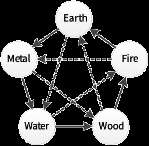
\includegraphics[]{pics/wuxing.jpeg}
\end{center}

A solid arrow from A to B means "A generates B", and a dotted arrow from A to B means "A overcomes B".

Now give you some pairs of different elements, please figure out the interaction between each pair.

\subsection{Input Format}

The first line contains an integer $N$, indicates the number of pairs of different elements.

Then $N$ lines follow. Each line contains a pair of strings $S_1$ and $S_2$, separated by a single space. Both $S_1$ and $S_2$ are one of the following five strings: "earth", "fire", "metal", "water", or "wood". $S_1$ and $S_2$ are different and indicate a pair of elements.

\subsection{Output Format}

For each pair of different elements $S_1$ and $S_2$, output a sentence in a single line in one of the four formats below, according to the interaction between them:
$S_1$ generates $S_2$.
$S_2$ generates $S_1$.
$S_1$ overcomes $S_2$.
$S_2$ overcomes $S_1$.

Note that for each sentence, there is a period (".") at the end and the first letter should be capitalized.

\subsection{Sample Input}
\begin{data}
2

earth water

earth fire
\end{data}
\subsection{Sample Output}
\begin{data}
Earth overcomes water.

Fire generates earth.
\end{data}

\clearpage{}